\section{Analiza kluczowych skryptów}
\subsection{Działanie skryptu start.sh}
\indent Skrypt jest wykonywany w powłoce Unix. Przed jego uruchomieniem, wymagana jest obecność katalogu \textit{\/home\/stos}, w którym docelowo zostaną stworzone nazwane potoki i katalog na pliki wyjściowe. Skrypt używa innego skryptu o nazwie \textit{setup.sh}, w którym nadawane są uprawnienia do plików \textit{start.sh} oraz \textit{stop.sh}, odpowiedzialnych za kolejno uruchamianie i zatrzymywanie kontenera. Dodatkowo modyfikowana jest wartość parametru jądra używanego w trakcie wykonywania, by każdy użytkownik mógł kontrolować wszystkie zdarzenia dotyczące wydajności systemu, poprzez ustawienie wartości „-1” parametru \textit{perf\_event\_paranoid} \cite{perf}. Po wykonaniu powyższych czynności wznawiana jest praca \textit{start.sh}, w której uruchamiany jest kontener na platformie kontenerowej Docker z podaną ilością zasobów obliczeniowych, zamontowanymi katalogami gospodarza oraz zmiennymi środowiskowymi. Utworzony kontener bazuje na obrazie Wine, który symuluje strukturę katalogową oraz umożliwia na uruchomienie plików wykonywalnych systemu operacyjnego Windows na systemie Linux.
\begin{figure}[!h]
	\begin{center}
		\resizebox{1.0\textwidth}{!} {
			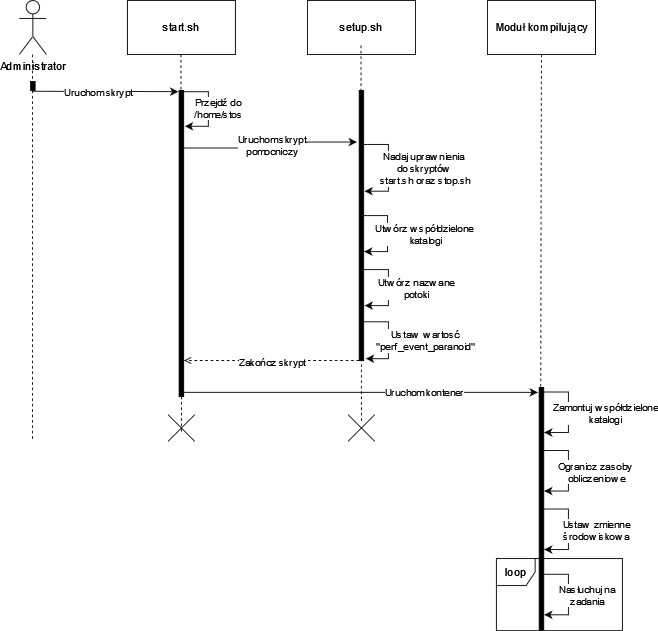
\includegraphics{img/2/start.png}
		}
		\caption[Diagram sekwenji skryptu start.sh]{Diagram sekwencji skryptu start.sh. Źródło własne.}
	\end{center}
\end{figure}

\subsection{Działanie skryptu startup.sh}
Podobnie jak \textit{start.sh}, \textit{startup.sh} wymaga obecności katalogu \textit{\/home\/stos} oraz jest wykonywany w powłoce Unix. Skrypt, oprócz przejścia do wyżej wspomnianego katalogu, używa skryptu \textit{serve.sh}. Podczas jego uruchomienia, następuje weryfikacja, czy w obecnym katalogu istnieją pliki wykonywalne i skrypty wymagane do poprawnego wykonania niezbędnych operacji, takich jak przesłanie i pobranie zadania. Kolejnym krokiem, jest uzyskanie adresu VPN, na który będą przesyłane pliki do oceny, poprzez wynik polecenia \textit{ip a show dev tap1}\cite{ip_addr}, które jest wywoływane w nieskończonej pętli, dopóki rezultat polecenia nie będzie zawierać pożądanego adresu. Następnie, uruchamiana jest nieskończona pętla odpytująca kolejkę zadań, która pobiera i waliduje zadanie, wybiera odpowiedni kompilator lub interpreter (w zależności od typu otrzymanego zgłoszenia), wykonuje i ocenia pojedyncze rozwiązanie studenta za pomocą procesów \textit{qapi} oraz \textit{sendresult}, przesyła wynik rozwiązania oraz czyści zbędne pliki. Proces kompilacji i oceny zadania, ze względu na mnogość operacji i używanych skryptów, zostanie pokazany w opisie skryptu \textit{handle-vc.sh}. 
\begin{figure}[!h]
	\begin{center}
		\resizebox{1.0\textwidth}{!} {
			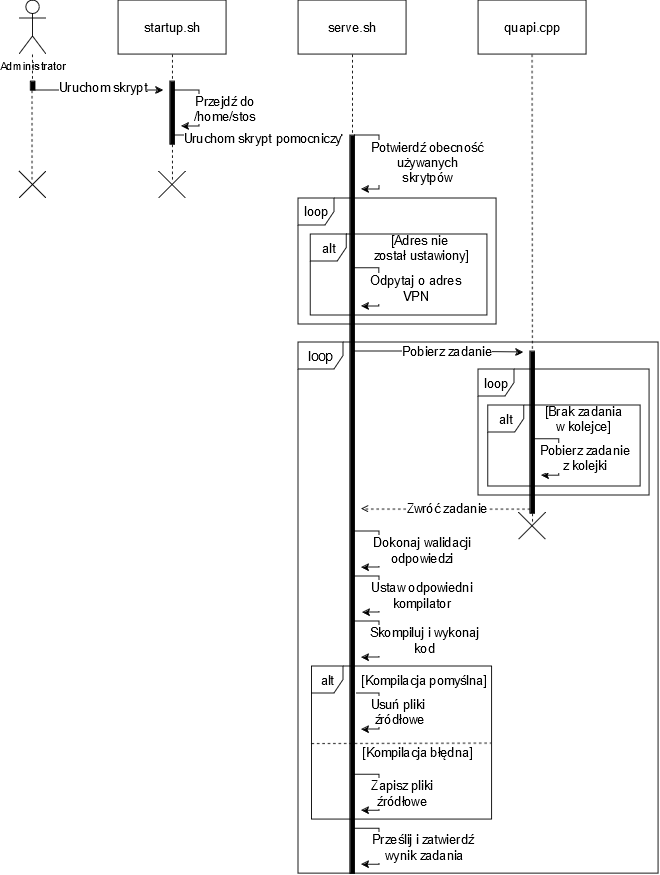
\includegraphics{img/2/startup.png}
		}
		\caption[Diagram sekwencji skryptu startup.sh]{Diagram sekwencji skryptu startup.sh. Źródło własne.}
	\end{center}
\end{figure}

\subsection{Działanie skryptu handle-vc.sh}
Jest to skrypt powłoki Uniksowej, odpowiedzialny za przesyłanie poleceń do modułu kompilującego oraz przesłanie oceny zadania. Jest używany w skrypcie \textit{serve.sh}. Istnieje kilka alternatywnych skryptów, pełniących analogiczną funkcję dla języków Python i Lua, oraz programów używających bibliotek Conio i SDL. Pierwszym krokiem, przed uruchomieniem kompilatora, jest synchronizacja danych ocenianego zadania, poprzez pobranie brakujących plików z serwera. Po zakończeniu procesu synchronizującego zmieniony zostaje używany katalog. W celu eliminacji potrzeby przekazywania zestawu parametrów otrzymanych z skryptu \textit{qapi} zostają one ustawione jako zmienna środowiskowa. Sterowanie zostaje przekazane do pliku \textit{runscript}, który jest plikiem wykonywalnym zawierającym szereg funkcji związanych z kompilacją, testowaniem oraz oceną zadania. Skrypt odczytuje parametr ze wcześniej ustawionej zmiennej środowiskowej, przekształca zadeklarowaną sekwencję testów do serii poleceń, które będą odczytane i wykonane w późniejszych krokach, tworzy pliki używane do zapisu wyniku kompilacji i metadanych o nazwie \textit{result.txt}, \textit{info.txt} i \textit{debug.txt}, waliduje je i zleca kompilacje skryptowi \textit{vc-compile.sh}. Skrypt przesyła sygnał do nazwanego potoku, który działający moduł kompilujący nasłuchuje. Gdy kompilacja jest zakończona, przesyłana jest informacja o jej rezultacie do wynikowego nazwanego potoku, na który oczekuje skrypt \textit{vc-compile.sh}. Wynik kompilacji zapisywany jest w odpowiednich plikach. Następnie wznawiana jest praca \textit{runscript}, który dokonuje oceny rozwiązania poprzez uruchamianie skompilowanego programu z zestawem danych wejściowych i porównania wyniku z oczekiwanym rezultatem. Ostatnim krokiem jest zapisanie wyniku w pliku oraz wypisanie informacji w przypadku wystąpienia błędu podczas oceny. Po wykonaniu czynności, \textit{handle-vc.sh} usuwa ustawioną na początku zmienną środowiskową, co kończy działanie tego aspektu systemu. Ze względu na brak plików nagłówkowych zawierających struktury danych i braku wiedzy na temat inżynierii wstecznej, dogłębna analiza części funkcjonalności, szczególnie synchronizacji oraz testowania, jest niewykonalna.
\begin{figure}[!h]
	\begin{center}
		\resizebox{0.9\textwidth}{!} {
			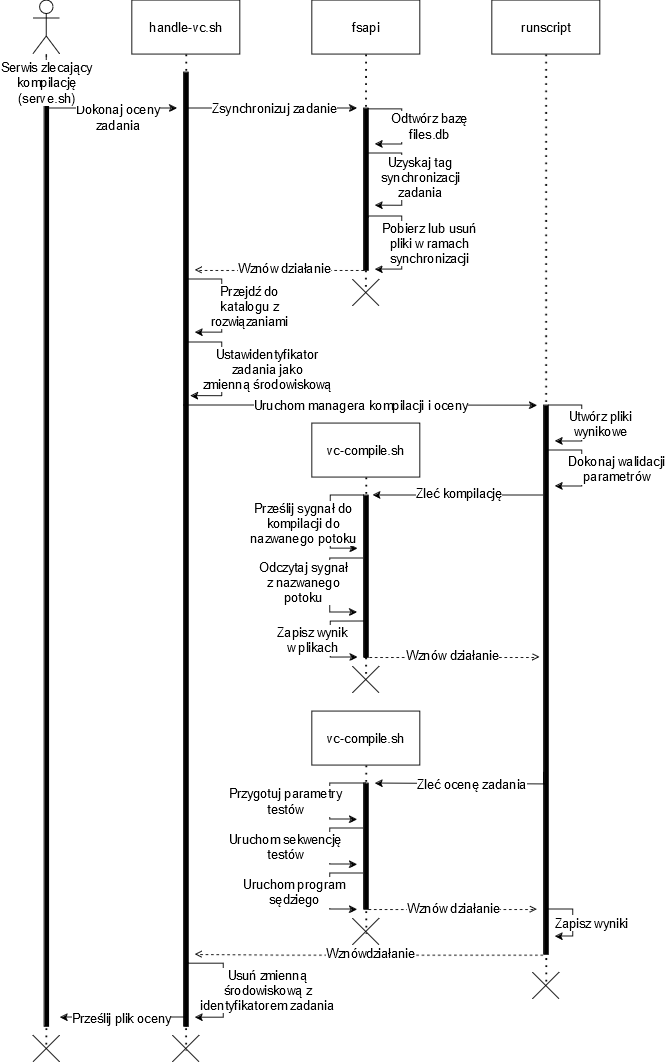
\includegraphics{img/2/handle.png}
		}
		\caption[Diagram sekwencji skryptu handle-vc.sh]{Diagram sekwencji skryptu handle-vc.sh. Źródło własne.}
	\end{center}
\end{figure}

\subsection{Działanie skryptu run.sh}
Skrypt jest punktem wejściowym dla kontenera modułu kompilującego. Znajduje się on na maszynie gospodarza i jest współdzielony z kontenerem, poprzez zamontowany dysk. Przy uruchomieniu, sprawdza, czy istnieją wymagane katalogi i pliki oraz rejestruję bibliotekę \textit{msdia140.dll}. Następnie, w nieskończonej pętli odczytuje komunikaty przesłane do nazwanego potoku \textit{input}. Zakładając, że skrypt wywołujący umieścił archiwum plików do kompilacji w odpowiednim katalogu, odczytuje go i rozpakowuje. Gdy walidacja plików przejdzie pomyślnie, wywoływany jest skrypt \textit{vc.sh} lub \textit{clang.sh}, na podstawie wartości pobranej z potoku. Ze względu na ich podobieństwo, przeanalizowane zostanie działanie \textit{vc.sh}. Skrypt ma za zadanie przygotować plik \textit{run.bat}, który będzie zawierać polecenia i wymagane parametry w celu kompilacji rozwiązania przesłanego przez studenta w kontenerze z obrazem \textit{Wine}. Wynik kompilacji jest zapisywany w nazwanym potoku wyjściowym.
\begin{figure}[!h]
	\begin{center}
		\resizebox{0.8\textwidth}{!} {
			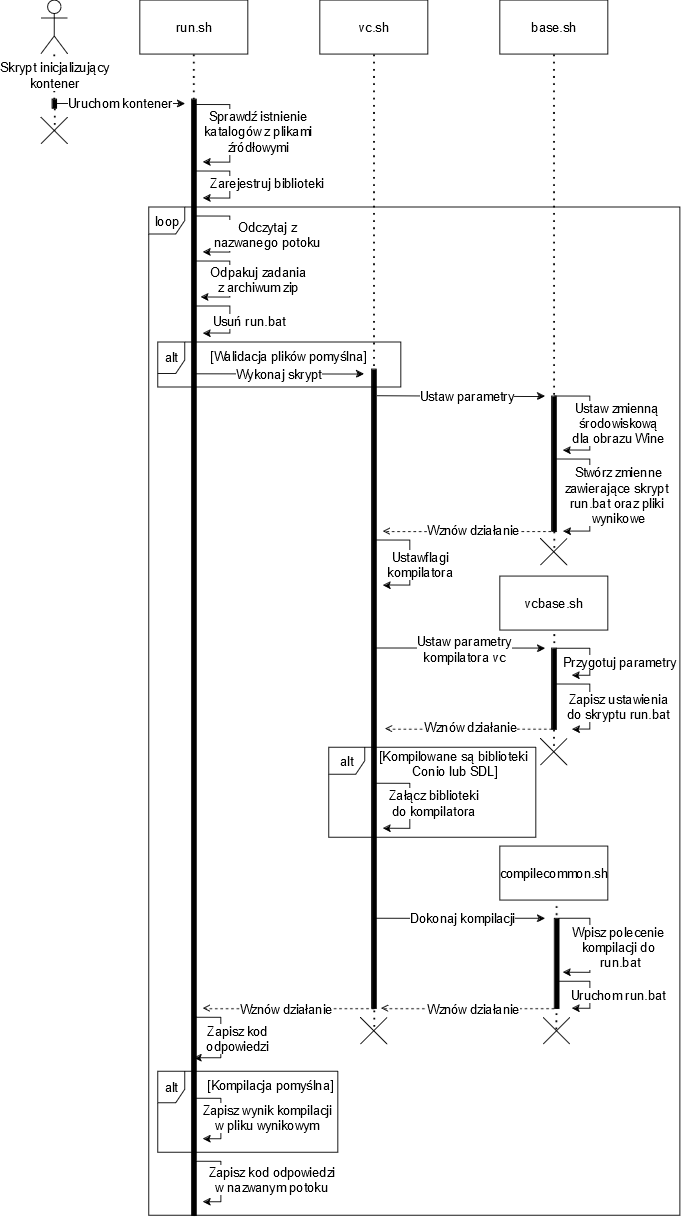
\includegraphics{img/2/run.png}
		}
		\caption[Diagram sekwencji skryptu run.sh]{Diagram sekwencji skryptu run.sh. Źródło własne.}
	\end{center}
\end{figure}